\documentclass[12pt]{article}
\usepackage{graphicx}
\usepackage{pgfplots}
\usepgfplotslibrary{fillbetween}
\usepgfplotslibrary{polar}
\usepackage{xfrac}
\pgfplotsset{compat=1.11}
\usetikzlibrary{calc}
\usepackage{setspace}
\usepackage{extsizes}
\usepackage{pgfplots}
\usepackage{float}
\usepackage{amsmath, amsthm, amssymb}    
\usepackage[margin=.5in]{geometry}
\usepackage[margin=.5in]{geometry}



\newcommand{\asa}{2}
\newcommand{\bsa}{0.5}
\newcommand{\csa}{0.5}


\title{\vspace{-2.0cm}Homework 7}
\author{Joanne Wardell}
\date{Thursday, September 20, 2018}
\begin{document}
\maketitle
\subsection*{Section 14.1}


\noindent 2.) $f(x, y) - \sin(xy)$\\\\
\noindent a.) $f(2, \frac{\pi}{6}) = \sin(\frac{2\pi}{6}) = \sin(\frac{\pi}{3}) = \frac{\sqrt{3}}{2}$\\\\
\noindent b.) $f(-3, \frac{\pi}{12}) = \sin(-\frac{3\pi}{12}) = -\sin(\frac{\pi}{4}) = -\frac{\sqrt{2}}{2}$\\\\
\noindent c.) $f(\pi, \frac{1}{4}) = \sin(\frac{\pi}{4}) = \frac{\sqrt{2}}{2}$\\\\
\noindent d.) $f(-\frac{\pi}{2}, -7) = \sin(\frac{7\pi}{2}) = -\sin(\frac{3\pi}{2}) = 1$\\\\\\\\

\noindent 6.) $f(x, y) = \ln{x^{2} + y^{2} - 4}$\\\\
\noindent $domain: \{ (x,y) \in \mathbb{R}^{2} | x^{2} + y^{2} > 4\}$\\

\begin{tikzpicture}
\begin{axis}[
    xmin=-6,xmax=6,
    ymin=-5,ymax=5,
    grid=both,
    grid style={line width=.1pt, draw=gray!10},
    major grid style={line width=.2pt,draw=gray!50},
    axis lines=middle,
    minor tick num=5,
    enlargelimits={abs=0.5},
    axis line style={latex-latex},
    ticklabel style={font=\tiny,fill=white},
    xlabel style={at={(ticklabel* cs:1)},anchor=north west},
    ylabel style={at={(ticklabel* cs:1)},anchor=south west},
    %restrict x to domain=-inf:0
]
\draw[dashed,black] (axis cs:0,0)circle [radius=2];
\end{axis}
\end{tikzpicture}\clearpage

\noindent 8.) $f(x, y) = \frac{\sin(xy)}{x^{2} + y^{2} - 25}$\\\\
\noindent $domain: \{ (x,y) \in \mathbb{R}^{2} | x^{2} + y^{2} > 25\}$\\
\begin{tikzpicture}
\begin{axis}[
    xmin=-6,xmax=6,
    ymin=-5,ymax=5,
    grid=both,
    grid style={line width=.1pt, draw=gray!10},
    major grid style={line width=.2pt,draw=gray!50},
    axis lines=middle,
    minor tick num=5,
    enlargelimits={abs=0.5},
    axis line style={latex-latex},
    ticklabel style={font=\tiny,fill=white},
    xlabel style={at={(ticklabel* cs:1)},anchor=north west},
    ylabel style={at={(ticklabel* cs:1)},anchor=south west},
    %restrict x to domain=-inf:0
]
\draw[dashed,black] (axis cs:0,0)circle [radius=5];
\end{axis}
\end{tikzpicture}\\\\



\noindent 14.) $f(x,y) = x^{2} + y^{2}$, \hspace{10pt} $c = 0, 1, 4, 9, 16, 25$\\
\noindent Below is a sketch of the level curves.\\
\begin{tikzpicture}
\begin{axis}[
    xmin=-6,xmax=6,
    ymin=-5,ymax=5,
    grid=both,
    grid style={line width=.1pt, draw=gray!10},
    major grid style={line width=.2pt,draw=gray!50},
    axis lines=middle,
    minor tick num=5,
    enlargelimits={abs=0.5},
    axis line style={latex-latex},
    ticklabel style={font=\tiny,fill=white},
    xlabel style={at={(ticklabel* cs:1)},anchor=north west},
    ylabel style={at={(ticklabel* cs:1)},anchor=south west},
    %restrict x to domain=-inf:0
]
\draw[black] (axis cs:0,0)circle [radius=0];
\draw[black] (axis cs:0,0)circle [radius=1];
\draw[black] (axis cs:0,0)circle [radius=2];
\draw[black] (axis cs:0,0)circle [radius=3];
\draw[black] (axis cs:0,0)circle [radius=4];
\draw[black] (axis cs:0,0)circle [radius=5];
\draw[black] (axis cs:0,0)circle [radius=6];
\draw[black] (axis cs:0,0)circle [radius=7];
\draw[black] (axis cs:0,0)circle [radius=8];
\end{axis}
\end{tikzpicture}\\\\


\noindent 32.) The level curves correspond to graph \textbf{b} and equation \textbf{i}.\\\\
\noindent 34.) The level curves correspond to graph \textbf{c} and equation \textbf{h}.\\\\
\noindent 36.) The level curves correspond to graph \textbf{e} and equation \textbf{j}.\clearpage
\noindent 44.) $f(x, y) = 6-2x-3y$\\
\noindent a.) Below is a sketch of the surface.\\
\begin{tikzpicture}
	\begin{axis}
		\addplot3[surf,]
    {-2*x-3*y + 6};

	\end{axis}
\end{tikzpicture}

\noindent b.) Below is an assortment of level curves in the function's domain.\\

\begin{tikzpicture}
\begin{axis}[
    xmin=-1.5,xmax=1.5,
    ymin=-1.5,ymax=1.5,
    grid=both,
    grid style={line width=.1pt, draw=gray!10},
    major grid style={line width=.2pt,draw=gray!50},
    axis lines=middle,
    minor tick num=5,
    enlargelimits={abs=0.5},
    axis line style={latex-latex},
    ticklabel style={font=\tiny,fill=white},
    xlabel style={at={(ticklabel* cs:1)},anchor=north west},
    ylabel style={at={(ticklabel* cs:1)},anchor=south west},
]
\addplot[color=black]{(-2/3)*x-(1/3)};
\addplot[color=black]{(-2/3)*x};
\addplot[color=black]{(-2/3)*x+(1/3)};
\addplot[color=black]{(-2/3)*x+(2/3)};
\addplot[color=black]{(-2/3)*x+1};

\end{axis}
\end{tikzpicture}\\


\noindent 48.) $f(x, y) = \sqrt{x^{2} +y^{2} -4}$\\
\noindent a.) Below is a sketch of the surface.\\
\begin{figure}[!h]
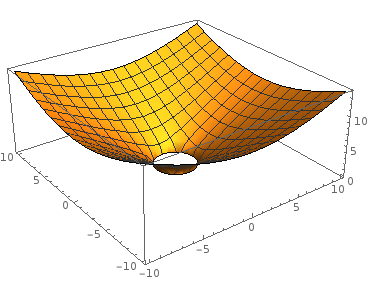
\includegraphics{graph1.png}
\end{figure}

\noindent b.) Below is an assortment of level curves in the function's domain.\\

\begin{tikzpicture}
\begin{axis}[
    xmin=-10,xmax=10,
    ymin=-10,ymax=10,
    grid=both,
    grid style={line width=.1pt, draw=gray!10},
    major grid style={line width=.2pt,draw=gray!50},
    axis lines=middle,
    minor tick num=5,
    enlargelimits={abs=0.5},
    axis line style={latex-latex},
    ticklabel style={font=\tiny,fill=white},
    xlabel style={at={(ticklabel* cs:1)},anchor=north west},
    ylabel style={at={(ticklabel* cs:1)},anchor=south west},
]

\draw[black] (axis cs:0,0)circle [radius=13];
\draw[black] (axis cs:0,0)circle [radius=20];
\draw[black] (axis cs:0,0)circle [radius=8];
\draw[black] (axis cs:0,0)circle [radius=5];
\draw[black] (axis cs:0,0)circle [radius=4];


\end{axis}
\end{tikzpicture}\\\\





\noindent 60.) $f(x, y, z) = \frac{x^{2}}{25} + \frac{y^{2}}{16} + \frac{z^{2}}{9}$\\
\noindent Below is a typical level surface for the function.\\

\begin{tikzpicture}
\begin{axis}
[view={135}{20},%colormap/blackwhite,
axis lines=center, axis on top,ticks=none,
set layers=default,axis equal,
xlabel={$x$}, ylabel={$y$}, zlabel={$z$},
xlabel style={anchor=south east},
ylabel style={anchor=south west},
zlabel style={anchor=south west},
enlargelimits,
tick align=inside,
domain=0:2.00,
samples=20, 
z buffer=sort,
]
\addplot3 [surf,opacity=0.4,domain=-1:0,
domain y=0:360] ({sin(y)*sqrt(1-x^2)},{2*cos(y)*sqrt(1-x^2)},{x});
\addplot3 [surf,opacity=0.4,domain=0:1,
domain y=0:360,on layer=axis foreground] ({sin(y)*sqrt(1-x^2)},{2*cos(y)*sqrt(1-x^2)},{x});
\end{axis}
\end{tikzpicture}



\subsection*{Section 14.2}

\noindent 4.) $\lim\limits_{(x,y) \to (3,4)} \sqrt{x^{2} + y^{2} - 1} = \sqrt{(3)^{2} + (4)^{2} -1} = \sqrt{24}$\\\\
\noindent 16.) $\lim\limits_{(x,y) \to (2,-4)} \frac{y+4}{x^{2}y -xy + 4x^{2} - 4x} 
\\\\= \lim\limits_{(x,y) \to (2,-4)} \frac{y+4}{xy(x-1)+4x(x-1)}
\\\\=\lim\limits_{(x,y) \to (2,-4)} \frac{y+4}{(x-1)(xy +4x)} 
\\\\=\lim\limits_{(x,y) \to (2,-4)} \frac{y+4}{(x-1)x(y +4)}
\\\\= \lim\limits_{(x,y) \to (2,-4)} \frac{1}{x(x-1)} = \frac{1}{2(2-1)} = \frac{1}{2}$\\\\\\

\noindent 26.) $\lim\limits_{P \to (1, -1, -1)}\frac{2xy+yz}{x^{2}+z^{2}} = \frac{2(-1)(-1) + (-1)(-1)}{(-1)^{2} + (-1)^{2}} = -\frac{1}{2}$
\clearpage
\noindent 32.) \\
\noindent a.) $f(x, y) = \frac{x+y}{x-y}$\\\\
\noindent The function is continuous for $\{ (x,y) \in \mathbb{R}^{2} | x \neq y$\\\\
\noindent b.) $f(x,y) = \frac{y}{x^{2} + 1}$\\\\
\noindent The function is continuous for all $ (x,y) \in \mathbb{R}^{2}$.\\\\
\noindent 36.) \\
\noindent a.) $f(x, y,z) = \ln(xyz)$\\\\
\noindent The function is continuous for $\{ (x,y,z) \in \mathbb{R}^{3} | xyz > 0\}$\\\\
\noindent b.) $f(x, y,z) = e^{x+y}\cos(z)$\\\\
\noindent The function is continuous for all $(x,y,z) \in \mathbb{R}^3$\\\\

\noindent 46.)$g(x,y) = \frac{x^{2}-y}{x -y}$\\\\
\noindent Using the two-path test for non-exsistence of a limit, we will show that the function has different limits along different paths as $(x,y)$ approaches a point.\\\\
\noindent Let $(x, y) \to (0,0)$ along any non-vertical line through the origin. 
\noindent Then, $y = mx$, where $m$ is the slope and $g(x,y)$ is:\\\\
$g(x,y) = g(x,mx)
\\\\\frac{x^{2} - mx}{x-mx}
\\\\\frac{x(x-m)}{x(1-m)}
\\\\\frac{x-m}{1-m}$\\\\
\noindent Thus, $g(x,y) \to \frac{-m}{1-m}$ as $(x,y)\to(0,0)$ along $y = mx$.\\\\
\noindent Since $m$ is any constant, the limit can approach different values along different paths. So, the limit doesn't exist.\\\\

\end{document}
